\newpage 
\section{Lecture 2: Finite Difference Method} 

Today's topics: 
\begin{itemize}
    \item Heat equation on $ \RR $ 
    \item Finite difference notation 
    \item Truncation error of simplest scheme equation  
\end{itemize}

\vspace{1em}
\hrule 
\vspace{1em} 


%────────────────────────────────────────
\begin{note}
The backward heat equation is ill-posed. Well-posedness means solutions exist, are unique and depends continuously on the ``data'', i.e., the initial condition $g$. 
\end{note}

\subsection{Heat equation with infinite domain}
%────────────────────────────────────────
Back to $u_t = u_{xx}$, but now $x\in \RR$ (infinite domain).  Now the b.c.'s are $ u(0)=0, u(\pi)=0 $ are replaced by requiring that $u(x,t)$ is bounded as $ x\to \pm \infty$ for each $t>0$.  This problem can be solved using the Fourier transform. The exact solution is: 
\[
    u(x,t) = \frac{1}{\sqrt{4\pi t} }\int_{-\infty}^{\infty} e^{-\frac{(x-\xi)^2}{4t}} g(\xi)\, d\xi.   
\]
The requirements on $g$ is that $g(x)$ should be continuous and bounded.  Here $G(x,t) = \frac{1}{\sqrt{4\pi t} }e^{-\frac{x^2}{4t}}$ is a Gaussian kernel. 


%────────────────────────────────────────
\begin{remark}
Here we have two observations: 
\begin{itemize}
    \item The exact solution is a smoothed-out version of the initial condition
    \item The value of $ u(x,t) $ at $x$ depends on all of $g(\xi)$ for every $t>0$. (Information travels infinitely fast, though the contribution from $g(\xi)$ decays super-exponentially with respect to $|x-\xi|$. 
\end{itemize}
\end{remark}
%────────────────────────────────────────

\subsection{Numerical method} 


%────────────────────────────────────────
\begin{note}
Question: WHy we use finite differences when we know the exact solution? 
\begin{itemize}
    \item Have to compute the integrals somehow (numerics still involved in evaluating exact solution) 
    \item These exact solutions don't generalize to more complicated geometries 
    \item Useful to develop intuition about the schemes on problems that you completely understand
\end{itemize}
\end{note}
%────────────────────────────────────────

Firstly, we have the discretization of time $t$ and position $x$ in fig~\ref{fig: 1-discre}.
\begin{figure}[H]
    \centering
    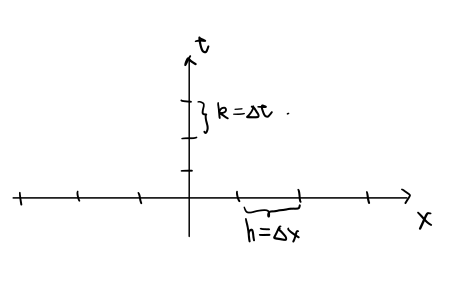
\includegraphics[width=0.5\textwidth]{figures/1-discretization.png}
    \label{fig: 1-discre}
\end{figure}
We also use the following notation: $u_j^n \approx u(jh, nk)$, where $u$ is the exact solution and $u_j^n$ is the numerical solution. For the initial condition, we set $u_j^0 = g(jh)$.  

The simplest scheme for $u_t = u_{xx}$ is the forward time centered space. We have the following approximations: 
\begin{align*}
   & u_t \approx \frac{u(x, t+ \Delta  t) - u(x,t)}{ \Delta t } = \frac{1}{k}\left[ u_j^{n+1} - u_j^n \right] = D_t^+ u_j^n \\ 
    &u_{xx} = \frac{u_x(x_j+\frac{h}{2},t_k) - u_x(x_j - \frac{h}{2},t_k)}{h}\approx \frac{1}{h}[\frac{u_{j+1}^n -u_j^n}{h}- \frac{u_j^n - u_{ j-1 } ^n}{h}] = \frac{1}{h^2}[u_{j+1}^n - 2u_j^n + u_{j-1}^n ] = D_x^+ D_x^- u_j^n. 
\end{align*}


%────────────────────────────────────────
\begin{definition}
[Finite difference]
\label{def: Finite difference}
Finite difference notations: 

\begin{itemize}
    \item $f(x)$ defined for $x\in \RR$, $f_j = f(x_j), x_j = jh$. 
    \item $D^+ f_j = \frac{f_{ j+1 } -f_j }{h}, \quad D^- f_j = \frac{f_j - f_{j-1}}{h}$ 
    \item $ D^0 f_j = \frac{f_{j+1}- f_{j-1}}{2h}, D^+D^- f_j = \frac{f_{j+1} - 2f_j + f_{j-1}}{h^2} $ 
\end{itemize}
Note that $f$ can mean $f(x)$ or $ \{f_j\}_{j=-\infty}^\infty $.  
\end{definition}
%────────────────────────────────────────

We should observe that 
\[
    D^+ D^- f_j = D^+ (D^-f_j) = \frac{1}{h}\left[ D^- f_{j+1} - D^- f_j \right]  = \frac{1}{h^2}[f_{j+1} -2f_j + f_{j-1}]. 
\]
Our scheme for $u_t = u_{xx}$ is 
\[
    D_t^+ u_j^n = D_x^+ D_x^- u_j^n. 
\]


